\section{Test Results} % (fold)
\label{sec:test_results}

\FloatBarrier \subsection{PC Incrementer} % (fold)
\label{sub:pc_incrementer} \FloatBarrier

The following observations correspond to the numbers in the \hyperref[sec:test_procedures]{Section \ref*{sec:test_procedures}} procedures for this part:

\begin{enumerate}
    \item The simulation using \emph{ModelSim} produced the output shown in \hyperref[fig:pcadder_output]{Figure \ref*{fig:pcadder_output}}.
    This output corresponds to \hyperref[tab:pcadder_vectors]{Table \ref*{tab:pcadder_vectors}} for each row, indicating the simulation passes.
    \item All test vectors as specified in \hyperref[tab:pcadder_vectors]{Table \ref*{tab:pcadder_vectors}} produced the corresponding outputs
\end{enumerate}

\begin{figure}
    %TODO output
    \caption{PC Incrementer \emph{ModelSim} Output\label{fig:pcadder_output}}
\end{figure}

% subsection pc_incrementer (end)

\FloatBarrier \subsection{Controller} % (fold)
\label{sub:controller} \FloatBarrier

The following observations correspond to the numbers in the \hyperref[sec:test_procedures]{Section \ref*{sec:test_procedures}} procedures for this part:

\begin{enumerate}
    \item The simulation using \emph{ModelSim} produced the output shown in \hyperref[fig:controller_output]{Figure \ref*{fig:controller_output}}.
    This output corresponds to \hyperref[fig:state_diagram]{Figure \ref*{fig:state_diagram}} for each row, indicating the simulation passes.
    \item The \emph{RTL Viewer} produced the result shown in \hyperref[fig:controller_rtl]{Figure \ref*{fig:controller_rtl}}.
    This is a reasonable result as it depicts a state machine with correct number and arrangement of states.
    \item All test vectors as specified in \hyperref[fig:state_diagram]{Figure \ref*{fig:state_diagram}} produced the corresponding outputs
\end{enumerate}

\begin{figure}
    %TODO output
    
\includegraphics[width=\textwidth]{images/controller_output.png}
    \caption{Controller \emph{ModelSim} Output\label{fig:controller_output}}
\end{figure}

\begin{figure}
    %TODO RTL
    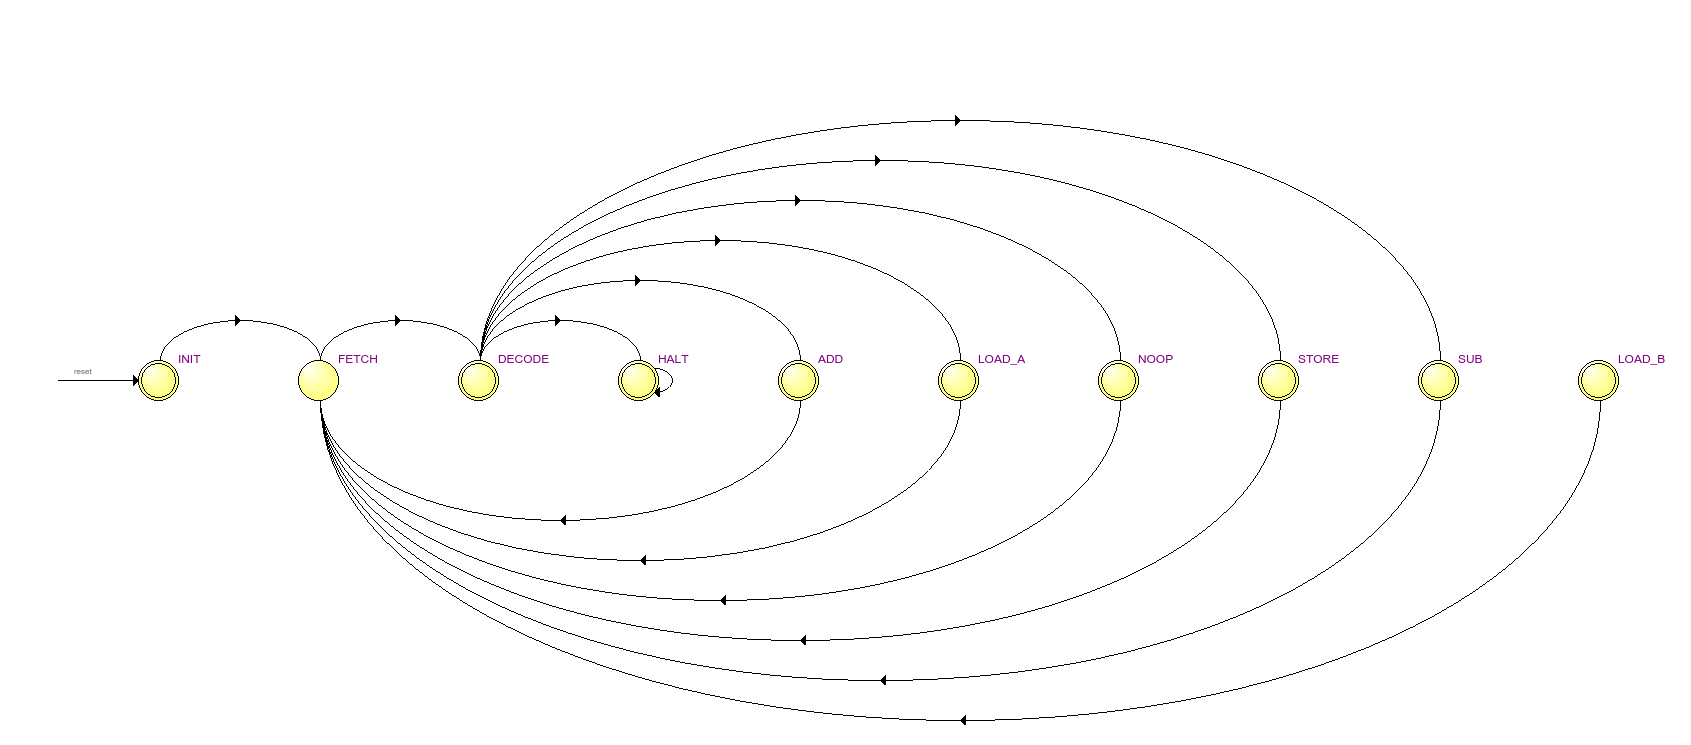
\includegraphics[width=\textwidth]{images/controller_rtl.png}
    \caption{Controller RTL View\label{fig:controller_rtl}}
\end{figure}

% subsection controller (end)

\FloatBarrier \subsection{Program Counter} % (fold)
\label{sub:program_counter} \FloatBarrier

The following observations correspond to the numbers in the \hyperref[sec:test_procedures]{Section \ref*{sec:test_procedures}} procedures for this part:

\begin{enumerate}
    \item The simulation using \emph{ModelSim} produced the output shown in \hyperref[fig:pc_output]{Figure \ref*{fig:pc_output}}.
    This output corresponds to \hyperref[tab:pc_vectors]{Table \ref*{tab:pc_vectors}} for each row, indicating the simulation passes.
    \item All test vectors as specified in \hyperref[tab:pc_vectors]{Table \ref*{tab:pc_vectors}} produced the corresponding outputs
\end{enumerate}

\begin{figure}
    %TODO output
    \caption{Program Counter \emph{ModelSim} Output\label{fig:pc_output}}
\end{figure}

% subsection program_counter (end)

\FloatBarrier \subsection{Instruction Register} % (fold)
\label{sub:instruction_register} \FloatBarrier

The following observations correspond to the numbers in the \hyperref[sec:test_procedures]{Section \ref*{sec:test_procedures}} procedures for this part:

\begin{enumerate}
    \item The simulation using \emph{ModelSim} produced the output shown in \hyperref[fig:ir_output]{Figure \ref*{fig:ir_output}}.
    This output corresponds to \hyperref[tab:ir_vectors]{Table \ref*{tab:ir_vectors}} for each row, indicating the simulation passes.
    \item All test vectors as specified in \hyperref[tab:ir_vectors]{Table \ref*{tab:ir_vectors}} produced the corresponding outputs
\end{enumerate}

\begin{figure}
    %TODO output
    \caption{Instruction Register \emph{ModelSim} Output\label{fig:ir_output}}
\end{figure}

% subsection instruction_register (end)

\FloatBarrier \subsection{Control Unit} % (fold)
\label{sub:control_unit} \FloatBarrier

The following observations correspond to the numbers in the \hyperref[sec:test_procedures]{Section \ref*{sec:test_procedures}} procedures for this part:

\begin{enumerate}
    \item The simulation using \emph{ModelSim} produced the output shown in \hyperref[fig:pcadder_output]{Figure \ref*{fig:cunit_output}}.
    This output corresponds to \hyperref[tab:cunit_vectors]{Table \ref*{tab:cunit_vectors}} for each row, indicating the simulation passes.
    \item All test vectors as specified in \hyperref[tab:cunit_vectors]{Table \ref*{tab:cunit_vectors}} produced the corresponding outputs
\end{enumerate}

\begin{figure}
    %TODO output
    \caption{Control Unit \emph{ModelSim} Output\label{fig:cunit_output}}
\end{figure}

% subsection control_unit (end)

\FloatBarrier \subsection{Datapath} % (fold)
\label{sub:datapath} \FloatBarrier

The following observations correspond to the numbers in the \hyperref[sec:test_procedures]{Section \ref*{sec:test_procedures}} procedures for this part:

\begin{enumerate}
    \item The simulation using \emph{ModelSim} produced the output shown in \hyperref[fig:datapath_output]{Figure \ref*{fig:datapath_output}}.
    This output corresponds to \hyperref[tab:datapath_vectors]{Table \ref*{tab:datapath_vectors}} for each row, indicating the simulation passes.
    \item All test vectors as specified in \hyperref[tab:datapath_vectors]{Table \ref*{tab:datapath_vectors}} produced the corresponding outputs
\end{enumerate}

\begin{figure}
    %TODO output
    \caption{Datapath \emph{ModelSim} Output\label{fig:datapath_output}}
\end{figure}

% subsection datapath (end)

\FloatBarrier \subsection{Processor} % (fold)
\label{sub:processor} \FloatBarrier

The following observations correspond to the numbers in the \hyperref[sec:test_procedures]{Section \ref*{sec:test_procedures}} procedures for this part:

\begin{enumerate}
    \item The simulation using \emph{ModelSim} produced the output shown in \hyperref[fig:processor_output]{Figure \ref*{fig:processor_output}}.
    This output corresponds to \hyperref[tab:processor_vectors]{Table \ref*{tab:processor_vectors}} for each row, indicating the simulation passes.
    \item All test vectors as specified in \hyperref[tab:processor_vectors]{Table \ref*{tab:processor_vectors}} produced the corresponding outputs
\end{enumerate}

\begin{figure}
    %TODO output
    \caption{Processor \emph{ModelSim} Output\label{fig:processor_output}}
\end{figure}

% subsection processor (end)

\FloatBarrier \subsection{Project} % (fold)
\label{sub:projects} \FloatBarrier

The following observations correspond to the numbers in the \hyperref[sec:test_procedures]{Section \ref*{sec:test_procedures}} procedures for this part:

\begin{enumerate}
    \item Compilation was successful, with the Flow Summary shown in \hyperref[fig:flow_summary]{Figure \ref*{fig:flow_summary}}.
    \item The project was downloaded to the DE2 board without errors.
    \item The displayed output was selectable as described in \hyperref[tab:display]{Table \ref*{tab:display}}.
\end{enumerate}

\begin{figure}
    %TODO flow summary
    
\includegraphics[width=\textwidth]{images/flow_summary.png}
    \caption{Flow Summary\label{fig:flow_summary}}
\end{figure}

% subsection projects (end)

% section test_results (end)